\documentclass[a4paper, 11pt]{article}           %{{{1
% basic packages                                  {{{2
\usepackage[T1]{fontenc}
\usepackage[scaled=0.975]{helvet}
\usepackage[utf8]{inputenc}
\usepackage{amsmath}
\usepackage{lastpage}
\usepackage{graphicx}
% marges {{{3
\addtolength{\voffset}{-1.8cm}
\addtolength{\textheight}{4cm}
\addtolength{\hoffset}{-2.5cm}
\addtolength{\textwidth}{4cm}
\addtolength{\headsep}{-0.5cm}
%}}}
\usepackage{fancyhdr}                                                           % configuration ci-dessous
% fancyhdr {{{3
\setlength{\headheight}{14.00pt}                                                %
\pagestyle{fancy}                                                               % Numérotation des pages
\renewcommand\footrulewidth{1pt}                                                %
\renewcommand\headrulewidth{1pt}                                                %
\fancyhead[L]{BP SN}                                                            %
\fancyhead[C]{arduino}                                                          %
\fancyhead[R]{introduction}                                                     %
\fancyfoot[L]{v 1.0 -- JB}                                                       %
\fancyfoot[C]{systèmes spécifiques}   %
\fancyfoot[R]{\thepage/\pageref{LastPage}}                                      %
% }}}
\usepackage{tcolorbox}
% ==== PROGRAMMATION
\usepackage{xcolor}                                                             %
\usepackage{listings}                                                           %
% listings                                        {{{3
\definecolor{mygreen}{rgb}{0,0.6,0}
\definecolor{mygray}{rgb}{0.5,0.5,0.5}
\definecolor{mymauve}{rgb}{0.58,0,0.82}
\definecolor{deepblue}{rgb}{0,0,0.5}
\definecolor{deepred}{rgb}{0.6,0,0}
\definecolor{deepgreen}{rgb}{0,0.5,0}
\lstset{%
% backgroundcolor=\color{white},   % choose the background color; you must add \usepackage{color} or \usepackage{xcolor}; should come as last argument
basicstyle=\footnotesize,        % the size of the fonts that are used for the code
% breakatwhitespace=false,         % sets if automatic breaks should only happen at whitespace
% breaklines=true,                 % sets automatic line breaking
% captionpos=b,                    % sets the caption-position to bottom
commentstyle=\color{mygreen},    % comment style
% deletekeywords={type},           % if you want to delete keywords from the given language
% emph={},                         % Custom highlighting
% emphstyle=\ttb\color{deepred}    % Custom highlighting style
% escapeinside={\%*}{*)},          % if you want to add LaTeX within your code
% extendedchars=true,              % lets you use non-ASCII characters; for 8-bits encodings only, does not work with UTF-8
frame=shadowbox,                 % adds a frame around the code {single, shadowbox}
% keepspaces=true,                 % keeps spaces in text, useful for keeping indentation of code (possibly needs columns=flexible)
keywordstyle=\color{blue},       % keyword style
language=C,                      % the language of the code {Python, C}
% morekeywords={*,...},            % if you want to add more keywords to the set
numbers=left,                    % numbers = (none, left, right)
% numbersep=5pt,                   % how far the line-numbers are from the code
% numberstyle=\tiny\color{mygray}, % the style that is used for the line-numbers
% otherkeywords={self},            % Add keywords here
% rulecolor=\color{black},         % if not set, the frame-color may be changed on line-breaks within not-black text (e.g. comments (green here))
rulesepcolor=\color{gray}        % shadowbox color
% showspaces=false,                % show spaces everywhere adding particular underscores; it overrides 'showstringspaces'
% showstringspaces=false,          % underline spaces within strings only
% showtabs=false,                  % show tabs within strings adding particular underscores
% stepnumber=1,                    % the step between two line-numbers. If it's 1, each line will be numbered
% stringstyle=\color{mymauve},     % string literal style
% tabsize=4,                       % sets default tabsize to 2 spaces
% title=\lstname                   % show the filename of files included with \lstinputlisting; also try caption instead of title
}
%}}}
%}}}

% Compteurs:                                     {{{2
\addtocounter{page}{0}
\newcounter{Q}
\newcounter{exoNB}
%}}}
% Longueur:                                      {{{2
\newlength{\longueurA}
\newlength{\longueurB}
\setlength{\parindent}{0pt}
\setlength{\parskip}{2pt}
\renewcommand{\baselinestretch}{1}
%}}}
% newcommand                                     {{{2
\newcommand{\question}{\stepcounter{Q} $\boxed{\arabic{Q}}$ }
\newcommand{\ligne}{\underline{\hspace{ \textwidth}} }
\newcommand{\LIGNE}{\vspace{2mm}\underline{\hspace{ \textwidth}} }
\newcommand{\reponse}{
  \par\nobreak
  \noindent\rule{0pt}{1.5\baselineskip}% Provides a larger gap between the preceding paragraph and the dots
  {\noindent\makebox[\linewidth]{\dotfill}\endgraf}% ... dotted lines ...
% \bigskip% Gap between dots and next paragraph
  }
\newcommand{\objectif}[1]{\textsc{\huge \textbf{Objectif :}\\ #1} }
\newcommand{\partie}[1]{\textsc{\Large #1} }
\newcommand{\exo}[1]{\stepcounter{exoNB}\textsc{\Large Exercice \arabic{exoNB} -- #1} }
\newcommand{\EXO}[2]{\stepcounter{exoNB}\textsc{\Large Exercice \arabic{exoNB} -- #1} \hfill \textbf{#2 points}}
\newcommand{\pb}[1] {\stepcounter{exoNB}\textsc{\Large Problème \arabic{exoNB} -- #1} }
\newcommand{\PB}[2] {\stepcounter{exoNB}\textsc{\Large Problème \arabic{exoNB} -- #1} \hfill \textbf{#2 points}}
%}}}
% Divers                                          {{{2
% listings                                        {{{3
%\definecolor{mygreen}{rgb}{0,0.6,0}
%\definecolor{mygray}{rgb}{0.5,0.5,0.5}
%\definecolor{mymauve}{rgb}{0.58,0,0.82}
%\definecolor{deepblue}{rgb}{0,0,0.5}
%\definecolor{deepred}{rgb}{0.6,0,0}
%\definecolor{deepgreen}{rgb}{0,0.5,0}
%\lstset{%
%        backgroundcolor=\color{white},   % choose the background color; you must add \usepackage{color} or \usepackage{xcolor}; should come as last argument
%        basicstyle=\footnotesize,        % the size of the fonts that are used for the code
%        breakatwhitespace=false,         % sets if automatic breaks should only happen at whitespace
%        breaklines=true,                 % sets automatic line breaking
%        captionpos=b,                    % sets the caption-position to bottom
%        commentstyle=\color{mygreen},    % comment style
%        deletekeywords={...},            % if you want to delete keywords from the given language
%        escapeinside={\%*}{*)},          % if you want to add LaTeX within your code
%        extendedchars=true,              % lets you use non-ASCII characters; for 8-bits encodings only, does not work with UTF-8
%        frame=single,                    % adds a frame around the code
%        keepspaces=true,                 % keeps spaces in text, useful for keeping indentation of code (possibly needs columns=flexible)
%        keywordstyle=\color{blue},       % keyword style
%        morekeywords={*,...},            % if you want to add more keywords to the set
%        numbers=left,                    % where to put the line-numbers; possible values are (none, left, right)
%        numbersep=5pt,                   % how far the line-numbers are from the code
%        numberstyle=\tiny\color{mygray}, % the style that is used for the line-numbers
%        rulecolor=\color{black},         % if not set, the frame-color may be changed on line-breaks within not-black text (e.g. comments (green here))
%        showspaces=false,                % show spaces everywhere adding particular underscores; it overrides 'showstringspaces'
%        showstringspaces=false,          % underline spaces within strings only
%        showtabs=false,                  % show tabs within strings adding particular underscores
%        stepnumber=2,                    % the step between two line-numbers. If it's 1, each line will be numbered
%        stringstyle=\color{mymauve},     % string literal style
%        tabsize=4,                       % sets default tabsize to 2 spaces
%        title=\lstname                   % show the filename of files included with \lstinputlisting; also try caption instead of title
%}
%\lstset{%
%        language=Python,                 % the language of the code
%        otherkeywords={self},            % Add keywords here
%        deletekeywords={type},           % if you want to delete keywords from the given language
%        emph={},                         % Custom highlighting
%        emphstyle=\ttb\color{deepred}    % Custom highlighting style
%}
%}}}

% PRL style line                                 {{{3
\newlength{\diamondrulelength}
\setlength{\diamondrulelength}{0.6\textwidth}
\newlength{\diamondrulethickness}
\setlength{\diamondrulethickness}{2pt}
\newcommand{\diamondrule}{\begin{center}\tikz{\fill[black] (0.5\diamondrulelength,0) -- (0,0.5\diamondrulethickness) -- (-0.5\diamondrulelength,0) -- (0,-0.5\diamondrulethickness) -- cycle;}\end{center}}
%}}}

% fixed with tabular                             {{{3
\usepackage{array}
\newcolumntype{L}[1]{>{\raggedright\let\newline\\\arraybackslash\hspace{0pt}}m{#1}}
\newcolumntype{C}[1]{>{\centering\let\newline\\\arraybackslash\hspace{0pt}}m{#1}}
\newcolumntype{R}[1]{>{\raggedleft\let\newline\\\arraybackslash\hspace{0pt}}m{#1}}
%}}}

%}}}
%}}}

% https://learn.adafruit.com/adafruit-arduino-lesson-1-blink/the-l-led
%

\begin{document}
\sffamily
\hfill Nom : {\noindent\makebox[5cm]{\dotfill}\endgraf}
\objectif{Première programmation de la carte}\\

\medskip

\partie{Le matériel}\\ %{{{1
- Une carte UNO + environnement de programmation arduino\\
- Une carte de prototypage et deux fils\\
- Deux résitances : 200 ohm et une un peu plus grande\\
- Une LED

%}}}

\bigskip

\partie{Présentation de l'arduino UNO}\\  %{{{1

Arduino, et son récent synonyme Genuino, est une marque qui couvre des cartes matériellement libres sur lesquelles se trouve un microcontrôleur (d'architecture Atmel AVR comme l'Atmega328p, et d'architecture ARM comme le Cortex-M3 pour l'Arduino Due). Les schémas de ces cartes sont publiés en licence libre. Cependant, certains composants, comme le microcontrôleur par exemple, ne sont pas sous licence libre.

Le microcontrôleur peut être programmé pour analyser et produire des signaux électriques, de manière à effectuer des tâches très diverses comme la domotique (le contrôle des appareils domestiques - éclairage, chauffage…), le pilotage d'un robot, de l'informatique embarquée, etc.


C'est une plate-forme basée sur une interface entrée/sortie simple. Il était destiné à l'origine principalement mais pas exclusivement à la programmation multimédia interactive en vue de spectacle ou d'animations artistiques, ce qui explique en partie la descendance de son environnement de développement de Processing, lui-même inspiré de l'environnement de programmation Wiring (l'un pensé pour la production d'applications impliquant des graphismes et l'autre pour pilotage de salles de spectacles).

\begin{figure}[!h]
\centering
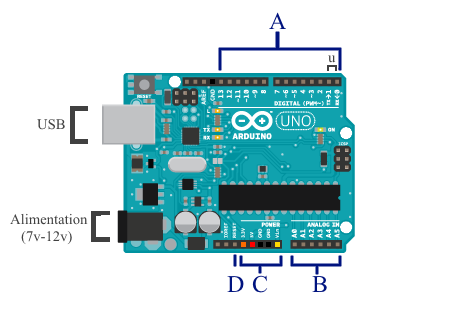
\includegraphics[width=0.85\linewidth]{CarteArduinoSimplifiee}
%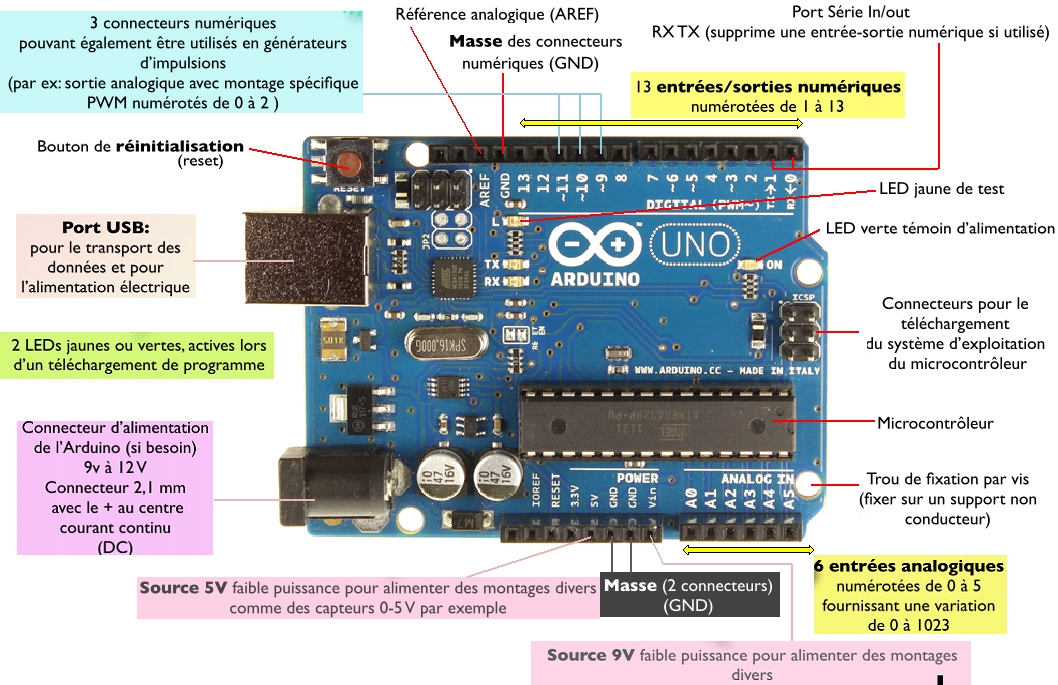
\includegraphics[width=\textwidth]{uno}
\caption{Principe des cartes arduino}
\label{CarteSimple}
\end{figure}


Les différentes versions des Arduino fonctionnent sous le même principe général :\\
\textbf{A : ce sont les broches dites numériques (0 ou 1)} ou " tout ou rien " ; elles offrent en sortie du 5 V et acceptent en entrée du 5 V sur le même principe.\\
- fonctions digitalWrite() et digitalRead()et pour les ports PWM analogWrite().\\
\textbf{B : ce sont les broches dites analogiques}, valeur entre 0 V et 5 V\\
- fonction analogRead()\\
\textbf{C : les différentes broches d'alimentation :}\\
-sortie 5 V (+)\\
-sortie 3,3 V (+)\\
-les masses (-)\\
-entrée reliée à l'alimentation (7 V-12 V)\\

Plus de détail sur les entrées sorties et leur programmation se trouve dans le très utile "PINOUT" montré sur la figure \ref{pinout}.
\begin{figure}[p]
\begin{center}
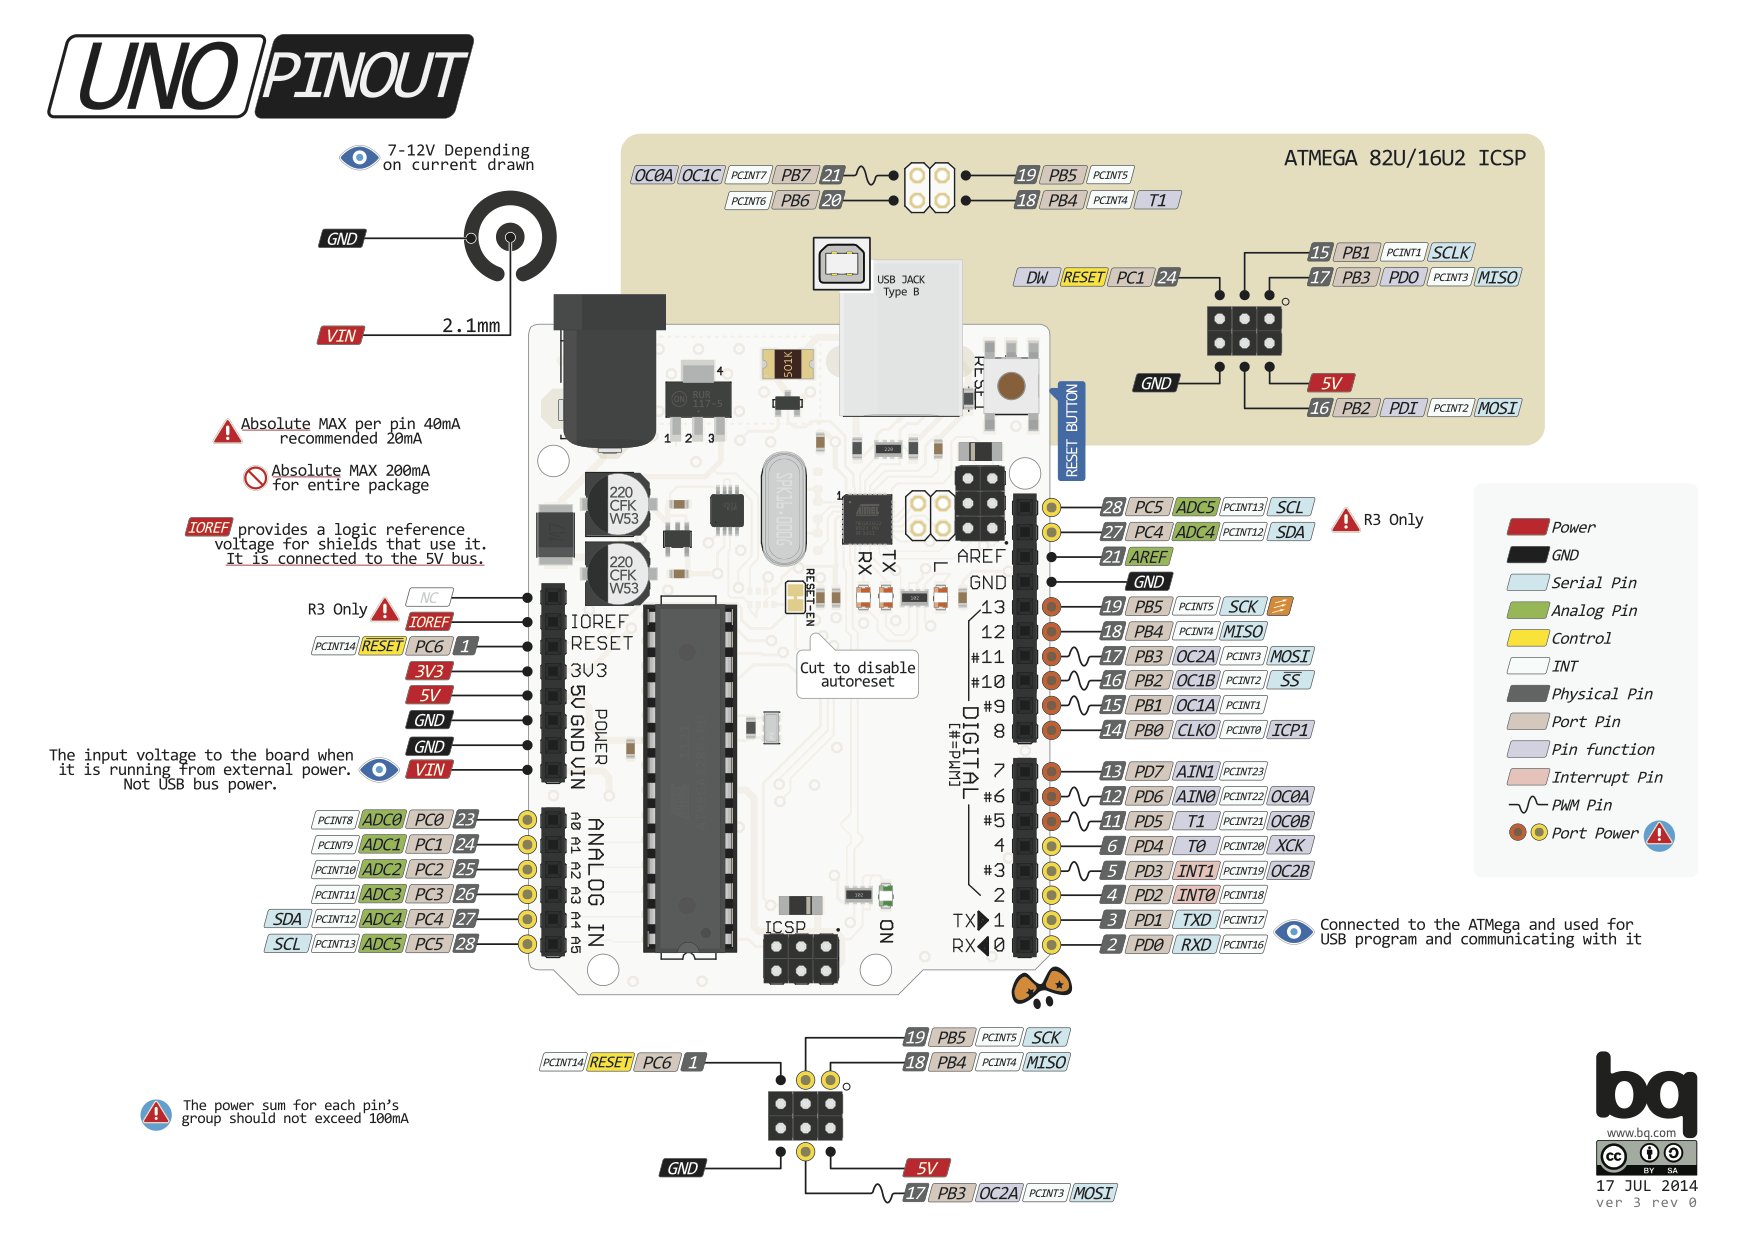
\includegraphics[angle=90, width=\textwidth]{UNOV3PDF}
\caption{Digramme des entrées-sorties.}
\label{pinout}
\end{center}
\end{figure}

%}}}

\bigskip

\partie{Familiarisation avec les spécifications techniques de la carte UNO et de son microcontrôleur ATMEGA 328P}\\ %{{{1

Pour cette partie, une recherche sur internet d'informations pertinente est nécessaire.\footnote{Un industriel, une encyclopédie, de la documentation technique, etc...}\\
\question Quelle est la tension de fonctionnent du microcontrôleur ?
\reponse

\question Quelle est la tension recommandée par le port d'alimentation noté en figure \ref{CarteSimple} ?
\reponse

\question Quel courant peut fournir une pin IO\footnote{pin se dit broche en français}\footnote{IO signifie In Out, entrée sortie en français} ?
\reponse

\question Combien y'a t'il de pin numériques ?
\reponse

\question Combien y'a t'il de pin analogiques ?
\reponse

\question Qu'elles soient sur la même carte électronique ou non, les puces électroniques peuvent s'échanger des informations. Plusieurs protocoles existent.
Donner la liste des protocoles de communication que le ATMEGA 328P permet-il ?
\reponse

%}}}

\bigskip

\partie{La carte arduino UNO : faire clignoter la LED 13}\\ %{{{1

\question Installer l'environnement de développement arduino depuis \texttt{www.arduino.cc}. Ouvrir le programme blink en le cherchant dans les menus. Sauvegarder une copie du programme blink sous un autre nom.

\question Si vous avez une carte UNO, nous devons peut-être installer un driver sur l'ordinateur ; c'est le cas si le composant qui fait l'adaptation entre l'USB (connecté au PC) et le port série du microcontrôleur est un CH340G. Dans les cartes originales, ce composant peut aussi bien être un atmel, un FTDI. Dans les cartes peu chères, un CH340G très peu cher est utilisé et nécessite l'installation d'un diver. Dans la figure 1, ce composant se localise entre le port USB et les deux LED Tx et Rx.
Sur la carte qui est à votre disposition, identifier le nom de ce composant. Identifier le nom de ce composant dans votre système d'exploitation.\\[0.2cm]

\question Si c'est un CH340, précisez la procédure d'installation du driver.
\reponse
\reponse

\texttt{Code source du programme Blink}
\begin{lstlisting}
// the setup function runs once when you press reset or power the board
void setup() {
  // initialize digital pin 13 as an output.
  pinMode(13, OUTPUT);
}

// the loop function runs over and over again forever
void loop() {
  digitalWrite(13, HIGH);   // turn the LED on (HIGH is the voltage level)
  delay(1000);              // wait for a second
  digitalWrite(13, LOW);    // turn the LED off by making the voltage LOW
  delay(1000);              // wait for a second
}
\end{lstlisting}

\question Téléverser le programme blink. Il faut configurer deux paramètres dans les menus : lesquels ?
\reponse

\question Est-ce que ce qui suit "//" est exécuté ?
\reponse

\question A quoi servent ces lignes ?
\reponse

\question Que signifie en français le commentaire \texttt{// the setup function runs once when you press reset or power the board }?
\reponse

\question Que signifie en français le commentaire \texttt{// the loop function runs over and over again forever }?

\question Pourquoi peut t'on l'appeler la LED L la LED de la pin 13 ?
\reponse

\question A quoi servent les LED TX et RX ? A quelles pins sont elles branchées ?
\reponse
\reponse

\question Quelle est la période de clignotement de la LED dans le programme blink tel qu'il est dans le menu examples ?
\reponse

\question Combiens de temps s'écoiule entre deux allumage de la LED de la pin 13 ?
\reponse

\question Quelle est donc la période de clignotement de la LED de la pin 13 ?
\reponse

\question Quelle est donc sa fréquence ?
\reponse

\question Pour un clignotement à 1 Hz, la période est de 1s. Quels paramètres changer pour l'implémenter ? Préciser son nom et sa valeur.
\reponse

\question De même pour 10 Hz.
\reponse

\question Faire clignoter la LED à 0,5 Hz, et vérifier avec un voltmètre que la broche de sortie de la carte UNO passe périodiquement de 0V et 5V.

\question Faire clignoter la LED à 0,5 Hz, et vérifier avec un voltmètre que la broche du microcontrôleur correspondante est périodiquement 0V ou 5V.

\question Faire clignoter la LED à 0,5 Hz, et vérifier avec un voltmètre que la tension aux bornes de la LED est d'environ 2V (ça dépend surtout de la couleur de la LED).

\medskip
\textbf{Bilan :}\\
- le fichier blink sauvegardé sous un autre nom ;\\
- le port série utilisé est identifié dans le gestionnaire de périphériques de l'ordinateur ; \\
- la LED clignote à 0,5Hz ;\\
- le voltmètre mesure bien 0V-5V sur une pin du microntrôleur, une pin de la carte ; \\
- le voltmètre mesure bien \~2V au bornes de la LED 13.\\
\tcbox{\textbf{Constatation professeur :} \hspace{5cm} }

%}}}

\bigskip

\partie{Connecter une LED externe}\\ %{{{1

\begin{figure}[!h]
\begin{center}
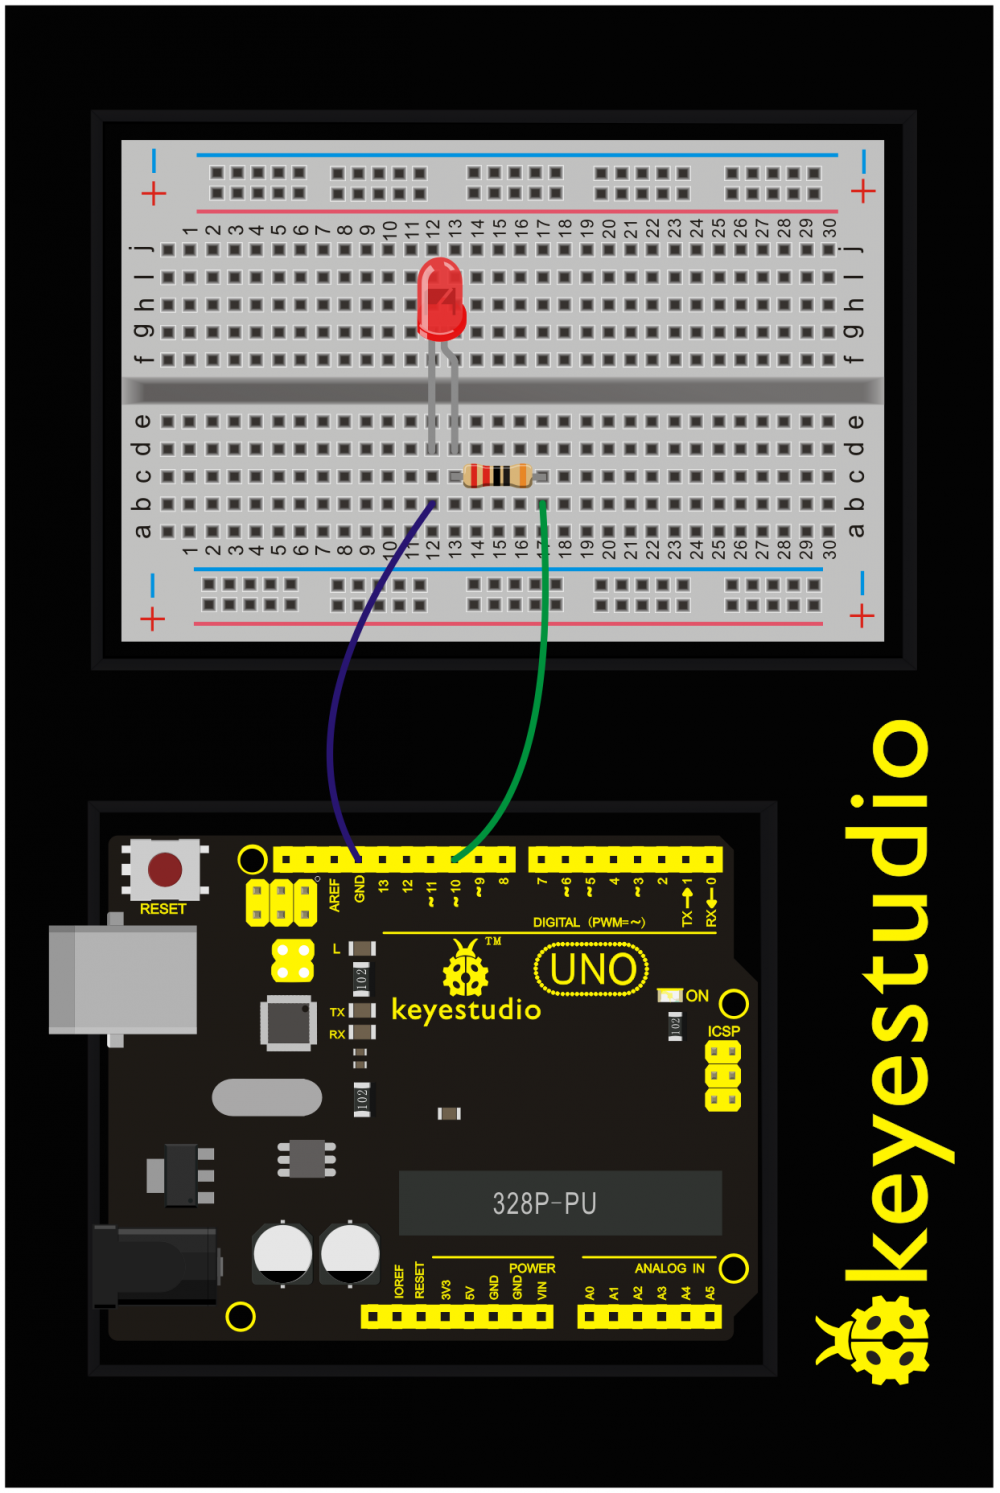
\includegraphics[height=\textwidth,angle=270]{CablageLED}\\
\caption{Cablage d'une LED externe}
\label{CablageLED}
\end{center}
\end{figure}

\texttt{Code source \#1}:
\begin{lstlisting}
int ledPin = 10; // define digital pin 10.
void setup() {
  pinMode(ledPin, OUTPUT);// define pin with LED connected as output.
}
void loop() {
  digitalWrite(ledPin, HIGH); // set the LED on.
  delay(1000); // wait for a second.
  digitalWrite(ledPin, LOW); // set the LED off.
  delay(1000); // wait for a second
}
\end{lstlisting}



\question Dans les conditions de ce montage, une valeur classique pour la résistance de polarisation de la LED est 220 ohm. Normalement ça dépend de la couleur de la LED, mais comme le microntrôleur et la carte sont bien protégés des erreurs, on se permet de faire à peu près. Quel est le calibre optimal pour la mesurer avec un multimètre ?
\reponse

\question Pourquoi ne convient-il pas d'utiliser un calibre en dessous ?
\reponse

\question Pourquoi ne convient-il pas d'utiliser un calibre en dessus ?
\reponse

\question Avec votre multimètre, mesurer la valeur exacte de la résitance que vous choisissez ?
\reponse

\question Implémentez le code \texttt{Code source \#1}.

\question Utilisez une valeur de resistance un peu plus grande. Qu'observez-vous ?
\reponse

\question Pour les deux résistances, saurez-vous calculer et mesurer les courants qui circulent dans la LED ? Précisez vos calculs et vos mesures.
\reponse


\textbf{Bilan:}\\
- resistance mesurée sur le bon calibre ;\\
- le montage marche ;\\
- observation avec une résistance plus grande.\\
\tcbox{\textbf{Constatation professeur :} \hspace{5cm} }
%}}}


\end{document}
